\documentclass{amsart}
%DIF LATEXDIFF DIFFERENCE FILE
%DIF DEL r.tex        Sun Aug 13 11:34:41 2023
%DIF ADD report.tex   Sat Jul 29 10:29:26 2023
\synctex=1

%=================================================================
% 
\newcount\DraftStatus  % 0 suppresses notes to selves in text
\DraftStatus=1   % TODO: set to 0 for final version
%=================================================================

%=================================================================
\usepackage{comment}
%=================================================================
%
\includecomment{JournalOnly}  
\includecomment{ConferenceOnly}  
\includecomment{TulipStyle}
%
%=================================================================
%=================================================================
% gitlatexdiff
%
%  https://gitlab.com/git-latexdiff/git-latexdiff
%=================================================================
%  git latexdiff HEAD  HEAD~5 --main templatex.tex
%  git latexdiff HEAD~1  --main templatex.tex
%  View pdf to see difference
%
%=================================================================
%
% Todo Notes for marginal comments
% 
%\newcount\DraftStatus  % 0 suppresses notes to selves in text
%\DraftStatus=1   % TODO: set to 0 for final version
\ifnum\DraftStatus=1
	\usepackage[draft,colorinlistoftodos,color=orange!30]{todonotes}
\else
	\usepackage[disable,colorinlistoftodos,color=blue!30]{todonotes}
\fi 
%\usepackage[disable]{todonotes} % notes not showed
%\usepackage[draft]{todonotes}   % notes showed
%
\makeatletter
 \providecommand\@dotsep{5}
 \def\listtodoname{List of Todos}
 \def\listoftodos{\@starttoc{tdo}\listtodoname}
 \makeatother
%
%=================================================================
%
\usepackage{color}
\newcommand{\draftnote}[3]{ 
	\todo[author=#2,color=#1!30,size=\footnotesize]{\textsf{#3}}	}
% TODO: add yourself here:
%
\newcommand{\gangli}[1]{\draftnote{blue}{GLi:}{#1}}
\newcommand{\qwu}[1]{\draftnote{red}{QWu:}{#1}}
\newcommand{\gliMarker}
	{\todo[author=GLi,size=\tiny,inline,color=blue!40]
	{Gang Li has worked up to here.}}
\newcommand{\qwuMarker}
	{\todo[author=QWu,size=\tiny,inline,color=red!40]
	{Qiong Wu has worked up to here.}}
%=================================================================

%=================================================================
%
% general packages
%  https://en.wikibooks.org/wiki/Category:Book:LaTeX
%  https://en.wikibooks.org/wiki/LaTeX/Package_Reference
%
%=================================================================
\usepackage{graphicx}
\usepackage{subfigure}
	
\usepackage{subcaption}
\graphicspath{{./figures/}{./graphics/}{./graphics/logos/}}

\usepackage{algorithm}
\usepackage{algorithmic}
\usepackage{breqn}
\usepackage{subcaption}
\usepackage{multirow}
\usepackage{psfrag}
\usepackage{url}
\usepackage[colorlinks,citecolor=blue]{hyperref}
%\usepackage{hyperref}
%\usepackage[colorlinks]{hyperref}
%\usepackage{cite}
\usepackage{cleveref}
\usepackage{booktabs}
\usepackage{rotating}
\usepackage{colortbl}
\usepackage{paralist}
%\usepackage{geometry}
\usepackage{epstopdf}
\usepackage{nag}
\usepackage{microtype}
\usepackage{siunitx}
\usepackage{nicefrac}
%\usepackage{breakurl}
\usepackage{fontawesome}
\usepackage{xcolor}
\usepackage{algorithmic}
\usepackage{algorithm}
\usepackage{multicol}
\usepackage{wrapfig}
\usepackage{todonotes}
\usepackage{tablefootnote}
\usepackage{threeparttable}
% \usepackage{bibunits} 
% for random text
\usepackage{cite}
\usepackage{lipsum}
\usepackage[english]{babel}
\usepackage[pangram]{blindtext}
% for tikz figures
\usepackage{tikz}
\usetikzlibrary{fit,positioning,arrows.meta,shapes,arrows}
%\tikzset{neuron/.style={circle,thick,fill=black!25,minimum size=17pt,inner sep=0pt},
%	input neuron/.style={neuron, draw,thick, fill=gray!30},
%	hidden neuron/.style={neuron,fill=white,draw},
%	hoz/.style={rotate=-90}}
%
%=================================================================



\begin{TulipStyle}
\usepackage[numbers]{natbib}
%=================================================================
%
% Version control information
%
%=================================================================
\usepackage{gitinfo2}
%=================================================================
\usepackage{fancyhdr}
\pagestyle{fancy}
\fancyhead{} % clear all header fields
\fancyhead[RO,LE]{\textsl{\rightmark}}
\fancyhead[LO,RE]{\ensuremath{\Rightarrow}
		\textbf{\textbf{[CONFIDENTIAL]}}\ensuremath{\Leftarrow}}
\fancyhead[CO,CE]{}
%=================================================================
\fancyfoot{} % clear all footer fields
\fancyfoot[CE,CO]{\textbf{\thepage}} 
\fancyfoot[LO,LE]{
\includegraphics[height=.9\headheight]
{./graphics/logos/tulip-logo.eps}
		\gitVtagn-\gitBranch\ (\gitCommitterDate)}
\fancyfoot[RO,RE]{Committed by: \textsl{\gitCommitterName}}

\setlength{\headheight}{12pt}
\renewcommand{\headrulewidth}{0.4pt}
\renewcommand{\footrulewidth}{0.4pt}
%=================================================================


%=================================================================
% for math notations
% ----------------------------------------------------------------
\usepackage{mathtools}
\usepackage{amsthm}
%
% THEOREMS -------------------------------------------------------
%
\newtheorem{thm}{Theorem}[section]
\newtheorem{cor}[thm]{Corollary}
\newtheorem{lem}[thm]{Lemma}
\newtheorem{prop}[thm]{Proposition}
\theoremstyle{definition}
\newtheorem{defn}[thm]{Definition}
\theoremstyle{remark}
\newtheorem{rem}[thm]{Remark}
\numberwithin{equation}{section}
% MATH -----------------------------------------------------------
\newcommand{\norm}[1]{\left\Vert#1\right\Vert}
\newcommand{\abs}[1]{\left\vert#1\right\vert}
\newcommand{\set}[1]{\left\{#1\right\}}
\newcommand{\Real}{\mathbb R}
\newcommand{\eps}{\varepsilon}
\newcommand{\To}{\longrightarrow}
\newcommand{\BX}{\mathbf{B}(X)}
% ----------------------------------------------------------------
\newcommand{\I}{{\cal I}}
\newcommand{\Id}{{\cal I} }
\newcommand{\Dc}{{\cal D}}
\newcommand{\J}{{\cal J}}
\newcommand{\Dn}{{\cal D}_n}
\newcommand{\Dd}{{\cal D}_n }
\renewcommand{\P}{{\cal P}}
\newcommand{\Nu}{{\cal N} }
\newcommand{\B}{{\cal B}}
\newcommand{\Bf}{{\bf B}}
\newcommand{\Y}{{\bf Y}}
\newcommand{\A}{{\cal A}}
% ----------------------------------------------------------------
\newcommand{\V}{{\cal V}}
\newcommand{\M}{{\cal M}}
\newcommand{\F}{{\cal F}}
\newcommand{\Fd}{{\cal F}}
\newcommand{\BF}{{\cal BF}_n}
\newcommand{\BFd}{{\cal BF}_n}
\newcommand{\TF}{{\cal TF}_n}
\newcommand{\TFd}{{\cal TF}_n}
%\newcommand{\G}{{\cal G}}
\newcommand{\X}{{\cal X}}
\newcommand{\E}{{\cal E}}
\newcommand{\K}{{\cal K}}
\newcommand{\T}{{\cal T}_n}
\renewcommand{\H}{{\cal H}}
% ----------------------------------------------------------------
\newtheorem{Remark}{Remark}
\newtheorem{proposition}{Proposition}
\newtheorem{theorem}{Theorem}
\newtheorem{lemma}{Lemma}
\newtheorem{corollary}{Corollary}
\newtheorem{example}{Example}
\newtheorem{definition}{Definition}
\newtheorem{Algorithms}{Algorithm}
% ----------------------------------------------------------------
\newcommand{\bu}{{\mathbf 1} }
\newcommand{\bo}{{\mathbf 0} }
\newcommand{\N}{\mbox{{\sl l}}\!\mbox{{\sl N}}}
% ----------------------------------------------------------------
\def\uint{[0,1]}
\def\proof{{\scshape Proof}. \ignorespaces}
\def\endproof{{\hfill \vbox{\hrule\hbox{%
   \vrule height1.3ex\hskip1.0ex\vrule}\hrule
  }}\par}
%
%=================================================================

\hypersetup
{
    pdfauthor={\gitAuthorName},
    pdfsubject={TULIP Lab},
    pdftitle={},
    pdfkeywords={TULIP Lab, Data Science},
%	bookmarks=true,  
}

\end{TulipStyle}




%=================================================================
%
%DIF PREAMBLE EXTENSION ADDED BY LATEXDIFF
%DIF UNDERLINE PREAMBLE %DIF PREAMBLE
\RequirePackage[normalem]{ulem} %DIF PREAMBLE
\RequirePackage{color}\definecolor{RED}{rgb}{1,0,0}\definecolor{BLUE}{rgb}{0,0,1} %DIF PREAMBLE
\providecommand{\DIFadd}[1]{{\protect\color{blue}\uwave{#1}}} %DIF PREAMBLE
\providecommand{\DIFdel}[1]{{\protect\color{red}\sout{#1}}}                      %DIF PREAMBLE
%DIF SAFE PREAMBLE %DIF PREAMBLE
\providecommand{\DIFaddbegin}{} %DIF PREAMBLE
\providecommand{\DIFaddend}{} %DIF PREAMBLE
\providecommand{\DIFdelbegin}{} %DIF PREAMBLE
\providecommand{\DIFdelend}{} %DIF PREAMBLE
\providecommand{\DIFmodbegin}{} %DIF PREAMBLE
\providecommand{\DIFmodend}{} %DIF PREAMBLE
%DIF FLOATSAFE PREAMBLE %DIF PREAMBLE
\providecommand{\DIFaddFL}[1]{\DIFadd{#1}} %DIF PREAMBLE
\providecommand{\DIFdelFL}[1]{\DIFdel{#1}} %DIF PREAMBLE
\providecommand{\DIFaddbeginFL}{} %DIF PREAMBLE
\providecommand{\DIFaddendFL}{} %DIF PREAMBLE
\providecommand{\DIFdelbeginFL}{} %DIF PREAMBLE
\providecommand{\DIFdelendFL}{} %DIF PREAMBLE
%DIF COLORLISTINGS PREAMBLE %DIF PREAMBLE
\RequirePackage{listings} %DIF PREAMBLE
\RequirePackage{color} %DIF PREAMBLE
\lstdefinelanguage{DIFcode}{ %DIF PREAMBLE
%DIF DIFCODE_UNDERLINE %DIF PREAMBLE
  moredelim=[il][\color{red}\sout]{\%DIF\ <\ }, %DIF PREAMBLE
  moredelim=[il][\color{blue}\uwave]{\%DIF\ >\ } %DIF PREAMBLE
} %DIF PREAMBLE
\lstdefinestyle{DIFverbatimstyle}{ %DIF PREAMBLE
	language=DIFcode, %DIF PREAMBLE
	basicstyle=\ttfamily, %DIF PREAMBLE
	columns=fullflexible, %DIF PREAMBLE
	keepspaces=true %DIF PREAMBLE
} %DIF PREAMBLE
\lstnewenvironment{DIFverbatim}{\lstset{style=DIFverbatimstyle}}{} %DIF PREAMBLE
\lstnewenvironment{DIFverbatim*}{\lstset{style=DIFverbatimstyle,showspaces=true}}{} %DIF PREAMBLE
%DIF END PREAMBLE EXTENSION ADDED BY LATEXDIFF

\begin{document}
%
%=================================================================
%
\DIFdelbegin %DIFDELCMD < \title[A Short Running Title]{%%%
\DIFdel{Title of This Paper}\DIFdelend \DIFaddbegin \title[FLIP01 PROJECT]{\DIFadd{FLIP01 PROJECT}\DIFaddend }%

\author{\DIFdelbegin \DIFdel{Author 1}\DIFdelend \DIFaddbegin \DIFadd{Jingbao Luo}\DIFaddend }
\DIFdelbegin %DIFDELCMD < \address[A.~1]{School of Computer Science,\\ 
%DIFDELCMD < Xi'an Shiyou University, Shaanxi 710065, China}%%%
\DIFdelend \DIFaddbegin \address[A.~1]{School of Economics and Management,\\ 
Nanjing University of Science and Technology, Nanjing 210094, China}\DIFaddend %
\DIFdelbegin %DIFDELCMD < \email[A.~1]{xxx@tulip.academy}
%DIFDELCMD < %%%
\DIFdelend \DIFaddbegin \email[A.~1]{jluo@tulip.academy}
\DIFaddend 

\DIFdelbegin %DIFDELCMD < \author{Gang Li}
%DIFDELCMD < \address[A.~2]{School of Information Technology \\
%DIFDELCMD < Deakin University, Geelong, VIC 3216, Australia}%%%
%DIF < 
%DIFDELCMD < \email[A.~2]{gang.li@deakin.edu.au}
%DIFDELCMD < 

%DIFDELCMD < \author{Author 3}
%DIFDELCMD < \address[A.~3]{School of Information Technology \\
%DIFDELCMD < Deakin University \\
%DIFDELCMD < Vic 3125, Australia}%%%
%DIF < 
%DIFDELCMD < \email[A.~3]{xxx@deakin.edu.au}
%DIFDELCMD < 

%DIFDELCMD < %%%
\DIFdelend %\thanks{Thanks to \ldots}%
\DIFdelbegin %DIFDELCMD < \subjclass{Artificial Intelligence}%%%
%DIF < 
\DIFdelend \date{\gitAuthorDate}%


\begin{abstract}
\DIFdelbegin \DIFdel{The abstract will be put here, .
...
}\DIFdelend \DIFaddbegin \DIFadd{This article utilizes the Isolation Forest algorithm to achieve credit card fraud detection with a recognition accuracy of 0.97 by continuously fine-tuning the algorithm.
}\DIFaddend \end{abstract}

\DIFdelbegin %DIFDELCMD < \keywords{Machine Learning, Data Mining, ...}%%%
\DIFdelend \DIFaddbegin \keywords{Machine Learning, Credit Card Data,IsolationForest}\DIFaddend %




\maketitle
\tableofcontents

\newpage
%=================================================================

%=================================================================
\section{Introduction}\label{sec-intro}



%DIF < \todo{Narrow down to a topic; Dig a hole; Fill the hole}
\DIFdelbegin %DIFDELCMD < \todo{Formula for Introduction}
%DIFDELCMD < 

%DIFDELCMD < %%%
%DIF < \gangli{``narrow in on topic'' reminds you 
%DIF < that readers and reviewers only know that this is a AI or HTM research paper (and maybe have read the title/abstract). 
%DIF < You need to help them figure out what topic and area of research paper this is. 
%DIF < You _don't_ need to wax poetic about the topic's importance.}
%DIFDELCMD < 

%DIFDELCMD < %%%
%DIF < \gangli{`dig a hole'' reminds you that 
%DIF < you need to convince the reader that there's a problem with the state of the world. 
%DIF < Prior work may exist but it's either missing something important or there's a missing opportunity. 
%DIF < The reader should be drooling for a bright future just out of reach.}
%DIFDELCMD < 

%DIFDELCMD < %%%
%DIF < \gangli{``fill the hole'' reminds you to show the reader 
%DIF < how and why the paper they're reading will fix these problems and deliver us into a better place. 
%DIF < You don't need a whirlwind summary of the technical details, 
%DIF < but you need readers convinced (and in a good mood) to keep reading.}
%DIFDELCMD < 

%DIFDELCMD < \gangli{A good paper introduction is fairly formulaic. 
%DIFDELCMD < If you follow a simple set of rules, 
%DIFDELCMD < you can write a very good introduction. 
%DIFDELCMD < The following outline can be varied. 
%DIFDELCMD < For example, 
%DIFDELCMD < you can use two paragraphs instead of one, 
%DIFDELCMD < or you can place more emphasis on one aspect of the intro than another. 
%DIFDELCMD < But in all cases, 
%DIFDELCMD < all of the points below need to be covered in an introduction, 
%DIFDELCMD < and in most papers, 
%DIFDELCMD < you don't need to cover anything more in an introduction.}
%DIFDELCMD < 

%DIFDELCMD < %%%
\DIFdelend %\todo{The importance of the area}
%\blindtext
\DIFdelbegin %DIFDELCMD < \todo{Motivation}
%DIFDELCMD < %%%
\DIFdel{At a high level, what is the problem area you are working in and why is it important? 
It is important to set the larger context here. Why is the problem of interest and importance to the larger community?
}\DIFdelend 

\DIFaddbegin \DIFadd{Credit card fraud refers to intentional acts of using forged or invalidated credit cards, impersonating others to deceive for financial gain, or engaging in malicious overdraft behavior using one's own credit card. There are three main forms of credit card fraud: card lost or stolen fraud, application fraud, and counterfeit credit card fraud. Among these fraud cases, over 60\% involve counterfeit credit cards, characterized by organized criminal activities that include stealing card information, manufacturing fake cards, selling counterfeit cards, and then using these fake cards to commit crimes for huge profits. Credit card fraud detection is a crucial method for banks to minimize losses.
}


\DIFaddend %\todo{The problems faced by most current methods}
%\blindtext
\DIFdelbegin %DIFDELCMD < \todo{What is the specific problem considered in this paper?}
%DIFDELCMD < %%%
\DIFdel{This paragraph narrows down the topic area of the paper. In the first paragraph you have established general context and importance. Here you establish specific context and background.
}\DIFdelend \DIFaddbegin 

\DIFadd{This article utilizes a dataset sourced from Kaggle to implement credit card fraud detection. The dataset contains transaction information of European cardholders during September 2013, conducted through credit cards. The dataset covers transactions that occurred within a span of two days, with a total of 284,807 transactions. Among these transactions, there were 492 cases of fraud, making the dataset highly imbalanced, where the positive class (fraudulent transactions) accounts for only 0.172%DIF >  of all transactions.
}\DIFaddend 

%DIF < \todo{What can be addressed by existing methods; Why those problems are challenges to existing methods?}
%DIF < \blindtext
\DIFdelbegin %DIFDELCMD < \todo{Contribution}
%DIFDELCMD < %%%
\DIFdel{"In this paper, we show that }\DIFdelend \DIFaddbegin \DIFadd{The original dataset has undergone anonymization and Principal Component Analysis (PCA) processing. The anonymous variables V1, V2, }\DIFaddend ...\DIFdelbegin \DIFdel{". This is the key paragraph in the intro - you summarize, in one paragraph, what are the main contributions of your paper given the context 
you have established in paragraphs }\DIFdelend \DIFaddbegin \DIFadd{, V28 represent the principal components obtained through PCA, and the only variables not subjected to PCA are Time and Amount. Time represents the time elapsed between each transaction and the first transaction in the dataset, measured in seconds, while Amount represents the transaction amount. The "Class" variable is a categorical variable, taking the value }\DIFaddend 1 \DIFdelbegin \DIFdel{and 2. 
What is the general approach taken? 
Why are the specific results significant? 
This paragraph must be really good}\DIFdelend \DIFaddbegin \DIFadd{when fraud occurs and 0 otherwise}\DIFaddend .

\DIFdelbegin \DIFdel{You should think about how to structure these one or 
two paragraph summaries of what your paper is all about. If there are two or three main results, then you might consider itemizing them with bullets or in test. 
}%DIFDELCMD < \begin{itemize}
\begin{itemize}%DIFAUXCMD
%DIFDELCMD < 	\item %%%
\item%DIFAUXCMD
\DIFdel{e.g.,First . ..
	}%DIFDELCMD < \item %%%
\item%DIFAUXCMD
\DIFdel{e.g., Second . ..
	}%DIFDELCMD < \item %%%
\item%DIFAUXCMD
\DIFdel{e.g., Third ...
}
\end{itemize}%DIFAUXCMD
%DIFDELCMD < \end{itemize}
%DIFDELCMD < %%%
\DIFdel{If the results fall broadly into two categories, you can bring out that distinction here. 
For example, "Our results are both theoretical and applied in nature. (two sentences follow, one each on theory and application)"
}\DIFdelend %DIF > \todo{What can be addressed by existing methods; Why those problems are challenges to existing methods?}
%DIF > \blindtext

\DIFaddbegin \DIFadd{This article utilizes a dataset sourced from Kaggle to implement credit card fraud detection. The dataset contains transaction information of European cardholders during September 2013, conducted through credit cards. The dataset covers transactions that occurred within a span of two days, with a total of 284,807 transactions. Among these transactions, there were 492 cases of fraud, making the dataset highly imbalanced, where the positive class (fraudulent transactions) accounts for only 0.172%DIF >  of all transactions.
}


\DIFaddend %\todo{What provides the motivation of this work? What are the research issues? What is the rationale of this work? }
%\blindtext
\DIFdelbegin %DIFDELCMD < \todo{At a high level what are the differences in what you are doing, and what others have done? }
%DIFDELCMD < %%%
\DIFdel{Keep this at a high level, you can refer to a future section where specific details and differences will be given. But it is important for the reader to know at a high level, what is new about this work compared to other work in the area.
}\DIFdelend 

%DIF < \todo{What we have done and what are the contributions.}
%DIF < \blindtext
\DIFdelbegin %DIFDELCMD < \todo{A roadmap for the rest of the paper}
%DIFDELCMD < %%%
\DIFdel{"The remainder of this paper is structured as follows. .." 
Give the reader a roadmap for the rest of the paper.
Avoid redundant phrasing, "In Section 2, In section 3, }\DIFdelend \DIFaddbegin \DIFadd{The original dataset has undergone anonymization and Principal Component Analysis (PCA) processing. The anonymous variables V1, V2, }\DIFaddend .\DIFdelbegin \DIFdel{.. In Section 4, }\DIFdelend .\DIFdelbegin \DIFdel{.. }\DIFdelend \DIFaddbegin \DIFadd{., V28 represent the principal components obtained through PCA, and the only variables not subjected to PCA are Time and Amount. Time represents the time elapsed between each transaction and the first transaction in the dataset, measured in seconds, while Amount represents the transaction amount. The }\DIFaddend "\DIFdelbegin \DIFdel{etc.
}%DIFDELCMD < 

%DIFDELCMD < \gangli{A few general tips:
%DIFDELCMD < Don't spend a lot of time into the introduction 
%DIFDELCMD < telling the reader about what you don't do in the paper. 
%DIFDELCMD < Be clear about what you do do.
%DIFDELCMD < Does each paragraph have a theme sentence that sets the stage for the entire paragraph? Are the sentences and topics in the paragraph all related to each other?}
%DIFDELCMD < 

%DIFDELCMD < \gangli{Does each paragraph have a theme 
%DIFDELCMD < sentence that sets the stage for the entire paragraph? 
%DIFDELCMD < Are the sentences and topics in the paragraph all related to each other?}
%DIFDELCMD < 

%DIFDELCMD < \gangli{Do all of your tenses match up in a paragraph?}
%DIFDELCMD < 

%DIFDELCMD < %%%
\DIFdel{Test citation~\mbox{%DIFAUXCMD
\cite{BL12J01}}\hskip0pt%DIFAUXCMD
. 
}%DIFDELCMD < \begin{JournalOnly}
%DIFDELCMD < %%%
\DIFdel{and ~\mbox{%DIFAUXCMD
\citep{BJL11J01} }\hskip0pt%DIFAUXCMD
or~\mbox{%DIFAUXCMD
\citet{BJL11J01}}\hskip0pt%DIFAUXCMD
.
}%DIFDELCMD < \end{JournalOnly}
%DIFDELCMD < 

%DIFDELCMD < %%%
\DIFdel{This is for~}%DIFDELCMD < \cref{tbl:overall-experiments}%%%
\DIFdel{, }%DIFDELCMD < \todo[fancyline]{Testing.}
%DIFDELCMD < %%%
\DIFdel{and this is for~}%DIFDELCMD < \cref{sec-conclusions}%%%
\DIFdel{.
}%DIFDELCMD < \todo[noline]{A note with no line back to the text.}%%%
%DIF < 
%DIFDELCMD < \gangli{This is comment from Gang.}
%DIFDELCMD < \qwu{Response from QW}
%DIFDELCMD < 

%DIFDELCMD < %%%
\DIFdel{Number:
}%DIFDELCMD < \num{123}%%%
\DIFdelend \DIFaddbegin \DIFadd{Class" variable is a categorical variable, taking the value 1 when fraud occurs and 0 otherwise}\DIFaddend .
\DIFdelbegin %DIFDELCMD < \numlist{10;30;50;70}%%%
\DIFdel{, }%DIFDELCMD < \numrange{10}{30}%%%
\DIFdel{,}%DIFDELCMD < \SIlist{10;30;45}{\metre}%%%
\DIFdel{,
and
}%DIFDELCMD < \SI{10}{\percent}
%DIFDELCMD < %%%
\DIFdelend 

\DIFdelbegin %DIFDELCMD < \missingfigure[figcolor=white]{Testing figcolor}
%DIFDELCMD < %%%
\DIFdelend \DIFaddbegin \DIFadd{The main implementation in this article is utilizing the Isolation Forest algorithm to achieve credit card fraud detection. By continuously fine-tuning the algorithm through parameter adjustments, the article aims to improve the algorithm's performance.
}\DIFaddend 



\DIFdelbegin %DIFDELCMD < \begin{ConferenceOnly}
%DIFDELCMD < %%%
\DIFdel{We have }%DIFDELCMD < \SI{10}{\hertz}%%%
\DIFdel{, }%DIFDELCMD < \si{\kilogram\metre\per\second}%%%
\DIFdel{,
the range: }%DIFDELCMD < \SIrange{10}{100}{\hertz}%%%
\DIFdel{.
$\nicefrac[]{1}{2}$.
}\DIFdelend \DIFaddbegin \section{\DIFadd{Method}} \label{sec-method}
\DIFadd{The Isolation Forest algorithm, proposed in 2008 by Liu Fei, Zhou Zhihua, and others, does not rely on distance or density metrics to describe the differences between samples and other samples. Instead, it directly characterizes the so-called isolation level. Therefore, this algorithm is simple, efficient, and widely used in the industry.
}\DIFaddend 

\DIFdelbegin %DIFDELCMD < \missingfigure{Make a sketch of the structure of a trebuchet.}
%DIFDELCMD < %%%
\DIFdelend \DIFaddbegin \DIFadd{The logic of the Isolation Forest algorithm is intuitive. It uses binary trees to split the data, and both sample selection and feature selection are performed using randomization. If a certain sample is an outlier, it may require very few iterations to be isolated.
}\DIFaddend 

\DIFdelbegin %DIFDELCMD < \end{ConferenceOnly}
%DIFDELCMD < %%%
\DIFdelend \DIFaddbegin \DIFadd{Isolation Forest algorithm code is ~}\cref{alg:iForest}\DIFadd{:
}\begin{algorithm}[!h]
	\caption{ \textit{\DIFadd{iForest}}}
	\label{alg:iForest}
	\renewcommand{\algorithmicrequire}{\textbf{Input:}}
	\renewcommand{\algorithmicensure}{\textbf{Output:}}
	\DIFaddend 

	\DIFdelbegin \DIFdel{For~}%DIFDELCMD < \cref{eq:test}%%%
\DIFdel{, as shown below:
}\DIFdelend \DIFaddbegin \begin{algorithmic}[1]
		\REQUIRE \DIFadd{$X$-Input data, $t$-number of trees ,$\varphi$ - subsampling size %DIF > %input
		}\ENSURE \DIFadd{a set of }\textit{\DIFadd{t iTRees}}   %DIF > %output
		\STATE \DIFadd{$\textbf{Initialize}$ $\textit{Forest}$
		}\STATE \DIFadd{set height limit $l = ceiling(log_{2}\varphi)$
		}\DIFaddend 

		\DIFdelbegin \begin{displaymath}\DIFdel{%DIFDELCMD < \label{eq:test}%%%
a = b \times \sqrt{ab}
}\end{displaymath}%DIFAUXCMD
\DIFdelend \DIFaddbegin \FOR{ $i = 1$ to $\textit{t}$} 
		\STATE \DIFadd{$X^{\prime}\!\leftarrow\!\cup(\textit{X,$\varphi$})$
		}\STATE \DIFadd{$\textit{Forest}\!\leftarrow\!\cup\textit{iTRees}(X^{\prime},0,\mathit{l})$
		}\ENDFOR
		\RETURN \DIFadd{$\textit{Forest}$
	}\end{algorithmic}
\end{algorithm}
\DIFaddend 

\DIFdelbegin %DIFDELCMD < \blindmathpaper
%DIFDELCMD < %%%
\DIFdelend \DIFaddbegin \section{\DIFadd{Data Exploration}} \label{sec-exploration}
\DIFaddend 


\DIFdelbegin \section{\DIFdel{Preliminaries}} %DIFAUXCMD
\addtocounter{section}{-1}%DIFAUXCMD
%DIFDELCMD < \label{sec-preliminaries}
%DIFDELCMD < %%%
\DIFdelend \DIFaddbegin \DIFadd{In this session, basic tools from pandas were utilized to perform data analysis and exploration. By analyzing the data, a more intuitive understanding was gained.
}\DIFaddend 

\DIFdelbegin %DIFDELCMD < \blindtext
%DIFDELCMD < %%%
\DIFdelend \DIFaddbegin \cref{tbl:data-description}\DIFadd{provides a basic overview of the data for each attribute, including measures such as the mean, maximum, minimum, and other indicators.
}\DIFaddend 

\DIFdelbegin %DIFDELCMD < \gliMarker  %%%
%DIF < TODO: GLi Here
%DIFDELCMD < 

%DIFDELCMD < %%%
\section{\DIFdel{Method}} %DIFAUXCMD
\addtocounter{section}{-1}%DIFAUXCMD
%DIFDELCMD < \label{sec-method}
%DIFDELCMD < 

%DIFDELCMD < \blindtext
%DIFDELCMD < \blindlist{itemize}[3]
%DIFDELCMD < \blinditemize
%DIFDELCMD < \blindenumerate
%DIFDELCMD < 

%DIFDELCMD < \blindmathtrue
%DIFDELCMD < \blindmathfalse
%DIFDELCMD < \blinddescription
%DIFDELCMD < 

%DIFDELCMD < \qwuMarker %%%
%DIF < TODO: QWu Here
%DIFDELCMD < 

%DIFDELCMD < %%%
\section{\DIFdel{Experiment and Analysis}} %DIFAUXCMD
\addtocounter{section}{-1}%DIFAUXCMD
%DIFDELCMD < \label{sec-experiment}
%DIFDELCMD < 

%DIFDELCMD < %%%
\DIFdelend \begin{table}  \centering
	\DIFaddbeginFL 

	\DIFaddendFL \caption{\DIFdelbeginFL \DIFdelFL{Precision Comparison on Event Detection Methods}\DIFdelendFL \DIFaddbeginFL \DIFaddFL{Data description}\DIFaddendFL }
	\DIFdelbeginFL %DIFDELCMD < \label{tbl:overall-experiments}
%DIFDELCMD <   \begin{tabular}{cccc}
%DIFDELCMD < \toprule
%DIFDELCMD <     %%%
%DIF <  after \\: \hline or \cline{col1-col2} \cline{col3-col4} ...
    \DIFdelendFL \DIFaddbeginFL \label{tbl:data-description}
	\resizebox{\textwidth}{!}
	{
		\begin{tabular}{cccccccccccccccccccccccccccccccc}
			\DIFaddendFL & \DIFdelbeginFL \DIFdelFL{OR Event Detection }\DIFdelendFL \DIFaddbeginFL \DIFaddFL{Time        }\DIFaddendFL & \DIFdelbeginFL \DIFdelFL{AC Event Detection }\DIFdelendFL \DIFaddbeginFL \DIFaddFL{V1          }\DIFaddendFL & \DIFdelbeginFL \DIFdelFL{TC Event Detection }\DIFdelendFL \DIFaddbeginFL \DIFaddFL{V2          }& \DIFaddFL{V3          }& \DIFaddFL{V4          }& \DIFaddFL{V5          }& \DIFaddFL{V6          }& \DIFaddFL{V7          }& \DIFaddFL{V8          }& \DIFaddFL{V9          }& \DIFaddFL{V10         }& \DIFaddFL{V11         }& \DIFaddFL{V12         }& \DIFaddFL{V13         }& \DIFaddFL{V14         }& \DIFaddFL{V15         }& \DIFaddFL{V16         }& \DIFaddFL{V17         }& \DIFaddFL{V18         }& \DIFaddFL{V19         }& \DIFaddFL{V20         }& \DIFaddFL{V21         }& \DIFaddFL{V22         }& \DIFaddFL{V23         }& \DIFaddFL{V24         }& \DIFaddFL{V25         }& \DIFaddFL{V26         }& \DIFaddFL{V27         }& \DIFaddFL{V28         }& \DIFaddFL{Amount      }& \DIFaddFL{Class       }\DIFaddendFL \\
			\DIFdelbeginFL %DIFDELCMD < \midrule
%DIFDELCMD <     %%%
\DIFdelFL{precision }\DIFdelendFL \DIFaddbeginFL \DIFaddFL{count }\DIFaddendFL & \DIFdelbeginFL \DIFdelFL{0.83 }\DIFdelendFL \DIFaddbeginFL \DIFaddFL{284807.0000 }\DIFaddendFL & \DIFdelbeginFL \DIFdelFL{0.69 }\DIFdelendFL \DIFaddbeginFL \DIFaddFL{284807.0000 }\DIFaddendFL & \DIFdelbeginFL \DIFdelFL{0.46 }\DIFdelendFL \DIFaddbeginFL \DIFaddFL{284807.0000 }& \DIFaddFL{284807.0000 }& \DIFaddFL{284807.0000 }& \DIFaddFL{284807.0000 }& \DIFaddFL{284807.0000 }& \DIFaddFL{284807.0000 }& \DIFaddFL{284807.0000 }& \DIFaddFL{284807.0000 }& \DIFaddFL{284807.0000 }& \DIFaddFL{284807.0000 }& \DIFaddFL{284807.0000 }& \DIFaddFL{284807.0000 }& \DIFaddFL{284807.0000 }& \DIFaddFL{284807.0000 }& \DIFaddFL{284807.0000 }& \DIFaddFL{284807.0000 }& \DIFaddFL{284807.0000 }& \DIFaddFL{284807.0000 }& \DIFaddFL{284807.0000 }& \DIFaddFL{284807.0000 }& \DIFaddFL{284807.0000 }& \DIFaddFL{284807.0000 }& \DIFaddFL{284807.0000 }& \DIFaddFL{284807.0000 }& \DIFaddFL{284807.0000 }& \DIFaddFL{284807.0000 }& \DIFaddFL{284807.0000 }& \DIFaddFL{284807.0000 }& \DIFaddFL{284807.0000 }\DIFaddendFL \\
			\DIFdelbeginFL \DIFdelFL{recall }\DIFdelendFL \DIFaddbeginFL \DIFaddFL{mean  }\DIFaddendFL & \DIFdelbeginFL \DIFdelFL{0.68 }\DIFdelendFL \DIFaddbeginFL \DIFaddFL{94813.8596  }\DIFaddendFL & \DIFdelbeginFL \DIFdelFL{0.48 }\DIFdelendFL \DIFaddbeginFL \DIFaddFL{0.0000      }\DIFaddendFL & \DIFdelbeginFL \DIFdelFL{0.36 }\DIFdelendFL \DIFaddbeginFL \DIFaddFL{0.0000      }& \DIFaddFL{0.0000      }& \DIFaddFL{0.0000      }& \DIFaddFL{0.0000      }& \DIFaddFL{0.0000      }& \DIFaddFL{0.0000      }& \DIFaddFL{0.0000      }& \DIFaddFL{0.0000      }& \DIFaddFL{0.0000      }& \DIFaddFL{0.0000      }& \DIFaddFL{0.0000      }& \DIFaddFL{0.0000      }& \DIFaddFL{0.0000      }& \DIFaddFL{0.0000      }& \DIFaddFL{0.0000      }& \DIFaddFL{0.0000      }& \DIFaddFL{0.0000      }& \DIFaddFL{0.0000      }& \DIFaddFL{0.0000      }& \DIFaddFL{0.0000      }& \DIFaddFL{0.0000      }& \DIFaddFL{0.0000      }& \DIFaddFL{0.0000      }& \DIFaddFL{0.0000      }& \DIFaddFL{0.0000      }& \DIFaddFL{0.0000      }& \DIFaddFL{0.0000      }& \DIFaddFL{88.3496     }& \DIFaddFL{0.0017      }\DIFaddendFL \\
			\DIFdelbeginFL \DIFdelFL{F-score }\DIFdelendFL \DIFaddbeginFL \DIFaddFL{std   }\DIFaddendFL & \DIFdelbeginFL \DIFdelFL{0.747 }\DIFdelendFL \DIFaddbeginFL \DIFaddFL{47488.1460  }\DIFaddendFL & \DIFdelbeginFL \DIFdelFL{0.57 }\DIFdelendFL \DIFaddbeginFL \DIFaddFL{1.9587      }\DIFaddendFL & \DIFdelbeginFL \DIFdelFL{0.4 }\DIFdelendFL \DIFaddbeginFL \DIFaddFL{1.6513      }& \DIFaddFL{1.5163      }& \DIFaddFL{1.4159      }& \DIFaddFL{1.3802      }& \DIFaddFL{1.3323      }& \DIFaddFL{1.2371      }& \DIFaddFL{1.1944      }& \DIFaddFL{1.0986      }& \DIFaddFL{1.0888      }& \DIFaddFL{1.0207      }& \DIFaddFL{0.9992      }& \DIFaddFL{0.9953      }& \DIFaddFL{0.9586      }& \DIFaddFL{0.9153      }& \DIFaddFL{0.8763      }& \DIFaddFL{0.8493      }& \DIFaddFL{0.8382      }& \DIFaddFL{0.8140      }& \DIFaddFL{0.7709      }& \DIFaddFL{0.7345      }& \DIFaddFL{0.7257      }& \DIFaddFL{0.6245      }& \DIFaddFL{0.6056      }& \DIFaddFL{0.5213      }& \DIFaddFL{0.4822      }& \DIFaddFL{0.4036      }& \DIFaddFL{0.3301      }& \DIFaddFL{250.1201    }& \DIFaddFL{0.0415      }\DIFaddendFL \\
			\DIFdelbeginFL %DIFDELCMD < \bottomrule
%DIFDELCMD < %%%
\DIFdelendFL \DIFaddbeginFL \DIFaddFL{min   }& \DIFaddFL{0.0000      }& \DIFaddFL{-56.4075    }& \DIFaddFL{-72.7157    }& \DIFaddFL{-48.3256    }& \DIFaddFL{-5.6832     }& \DIFaddFL{-113.7433   }& \DIFaddFL{-26.1605    }& \DIFaddFL{-43.5572    }& \DIFaddFL{-73.2167    }& \DIFaddFL{-13.4341    }& \DIFaddFL{-24.5883    }& \DIFaddFL{-4.7975     }& \DIFaddFL{-18.6837    }& \DIFaddFL{-5.7919     }& \DIFaddFL{-19.2143    }& \DIFaddFL{-4.4989     }& \DIFaddFL{-14.1299    }& \DIFaddFL{-25.1628    }& \DIFaddFL{-9.4987     }& \DIFaddFL{-7.2135     }& \DIFaddFL{-54.4977    }& \DIFaddFL{-34.8304    }& \DIFaddFL{-10.9331    }& \DIFaddFL{-44.8077    }& \DIFaddFL{-2.8366     }& \DIFaddFL{-10.2954    }& \DIFaddFL{-2.6046     }& \DIFaddFL{-22.5657    }& \DIFaddFL{-15.4301    }& \DIFaddFL{0.0000      }& \DIFaddFL{0.0000      }\\
			\DIFaddFL{0.25  }& \DIFaddFL{54201.5000  }& \DIFaddFL{-0.9204     }& \DIFaddFL{-0.5985     }& \DIFaddFL{-0.8904     }& \DIFaddFL{-0.8486     }& \DIFaddFL{-0.6916     }& \DIFaddFL{-0.7683     }& \DIFaddFL{-0.5541     }& \DIFaddFL{-0.2086     }& \DIFaddFL{-0.6431     }& \DIFaddFL{-0.5354     }& \DIFaddFL{-0.7625     }& \DIFaddFL{-0.4056     }& \DIFaddFL{-0.6485     }& \DIFaddFL{-0.4256     }& \DIFaddFL{-0.5829     }& \DIFaddFL{-0.4680     }& \DIFaddFL{-0.4837     }& \DIFaddFL{-0.4988     }& \DIFaddFL{-0.4563     }& \DIFaddFL{-0.2117     }& \DIFaddFL{-0.2284     }& \DIFaddFL{-0.5424     }& \DIFaddFL{-0.1618     }& \DIFaddFL{-0.3546     }& \DIFaddFL{-0.3171     }& \DIFaddFL{-0.3270     }& \DIFaddFL{-0.0708     }& \DIFaddFL{-0.0530     }& \DIFaddFL{5.6000      }& \DIFaddFL{0.0000      }\\
			\DIFaddFL{0.5   }& \DIFaddFL{84692.0000  }& \DIFaddFL{0.0181      }& \DIFaddFL{0.0655      }& \DIFaddFL{0.1798      }& \DIFaddFL{-0.0198     }& \DIFaddFL{-0.0543     }& \DIFaddFL{-0.2742     }& \DIFaddFL{0.0401      }& \DIFaddFL{0.0224      }& \DIFaddFL{-0.0514     }& \DIFaddFL{-0.0929     }& \DIFaddFL{-0.0328     }& \DIFaddFL{0.1400      }& \DIFaddFL{-0.0136     }& \DIFaddFL{0.0506      }& \DIFaddFL{0.0481      }& \DIFaddFL{0.0664      }& \DIFaddFL{-0.0657     }& \DIFaddFL{-0.0036     }& \DIFaddFL{0.0037      }& \DIFaddFL{-0.0625     }& \DIFaddFL{-0.0295     }& \DIFaddFL{0.0068      }& \DIFaddFL{-0.0112     }& \DIFaddFL{0.0410      }& \DIFaddFL{0.0166      }& \DIFaddFL{-0.0521     }& \DIFaddFL{0.0013      }& \DIFaddFL{0.0112      }& \DIFaddFL{22.0000     }& \DIFaddFL{0.0000      }\\
			\DIFaddFL{0.75  }& \DIFaddFL{139320.5000 }& \DIFaddFL{1.3156      }& \DIFaddFL{0.8037      }& \DIFaddFL{1.0272      }& \DIFaddFL{0.7433      }& \DIFaddFL{0.6119      }& \DIFaddFL{0.3986      }& \DIFaddFL{0.5704      }& \DIFaddFL{0.3273      }& \DIFaddFL{0.5971      }& \DIFaddFL{0.4539      }& \DIFaddFL{0.7396      }& \DIFaddFL{0.6182      }& \DIFaddFL{0.6625      }& \DIFaddFL{0.4931      }& \DIFaddFL{0.6488      }& \DIFaddFL{0.5233      }& \DIFaddFL{0.3997      }& \DIFaddFL{0.5008      }& \DIFaddFL{0.4589      }& \DIFaddFL{0.1330      }& \DIFaddFL{0.1864      }& \DIFaddFL{0.5286      }& \DIFaddFL{0.1476      }& \DIFaddFL{0.4395      }& \DIFaddFL{0.3507      }& \DIFaddFL{0.2410      }& \DIFaddFL{0.0910      }& \DIFaddFL{0.0783      }& \DIFaddFL{77.1650     }& \DIFaddFL{0.0000      }\\
			\DIFaddFL{max   }& \DIFaddFL{172792.0000 }& \DIFaddFL{2.4549      }& \DIFaddFL{22.0577     }& \DIFaddFL{9.3826      }& \DIFaddFL{16.8753     }& \DIFaddFL{34.8017     }& \DIFaddFL{73.3016     }& \DIFaddFL{120.5895    }& \DIFaddFL{20.0072     }& \DIFaddFL{15.5950     }& \DIFaddFL{23.7451     }& \DIFaddFL{12.0189     }& \DIFaddFL{7.8484      }& \DIFaddFL{7.1269      }& \DIFaddFL{10.5268     }& \DIFaddFL{8.8777      }& \DIFaddFL{17.3151     }& \DIFaddFL{9.2535      }& \DIFaddFL{5.0411      }& \DIFaddFL{5.5920      }& \DIFaddFL{39.4209     }& \DIFaddFL{27.2028     }& \DIFaddFL{10.5031     }& \DIFaddFL{22.5284     }& \DIFaddFL{4.5845      }& \DIFaddFL{7.5196      }& \DIFaddFL{3.5173      }& \DIFaddFL{31.6122     }& \DIFaddFL{33.8478     }& \DIFaddFL{25691.1600  }& \DIFaddFL{1.0000     
		}\DIFaddendFL \end{tabular}
	\DIFaddbeginFL }
\DIFaddendFL \end{table}

\DIFdelbegin \section{\DIFdel{Conclusions}} %DIFAUXCMD
\addtocounter{section}{-1}%DIFAUXCMD
%DIFDELCMD < \label{sec-conclusions}
%DIFDELCMD < %%%
\DIFdelend \DIFaddbegin \DIFadd{From the perspective of fraud occurrence, the data was visualized as shown in }\cref{fig:fraud data}\DIFadd{. It can be observed that the instances of fraud are significantly fewer than non-fraudulent cases, indicating the presence of data imbalance.
}\DIFaddend 

\DIFdelbegin %DIFDELCMD < \blindtext
%DIFDELCMD < %%%
\DIFdelend \DIFaddbegin \begin{figure}[H]
	\centering
	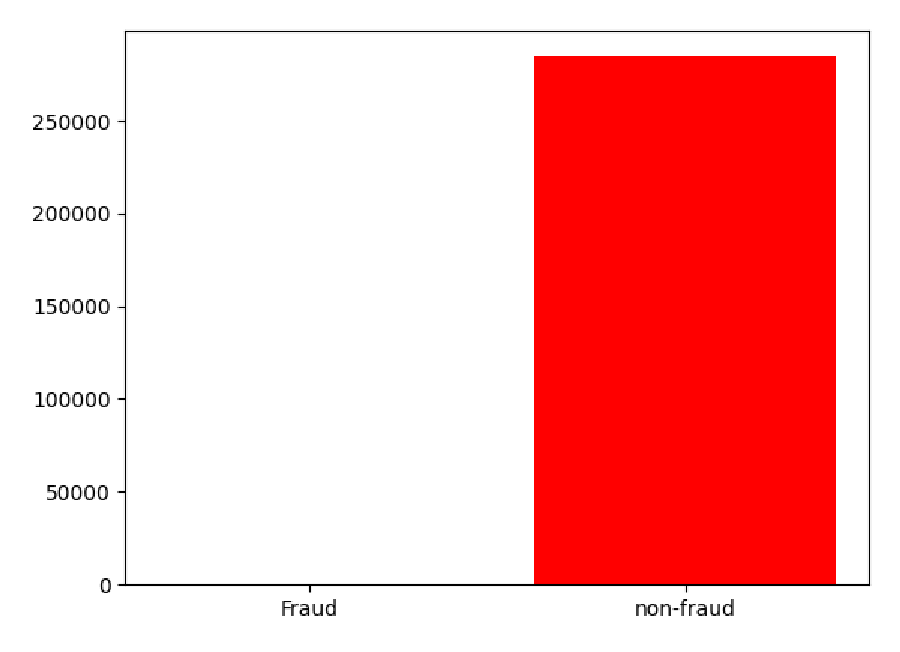
\includegraphics[width=0.7\textwidth]{figures/fraud.eps}
	\caption{\DIFaddFL{fraud or no fraud}}
	\label{fig:fraud data}
\end{figure}
\DIFaddend 

\DIFdelbegin \section*{\DIFdel{Acknowledgement}}
%DIFAUXCMD
\DIFdelend \DIFaddbegin \cref{fig:correlation} \DIFadd{is a heatmap of correlations, representing the correlation of each attribute with fraud.From the figure, it can be seen that the individual attributes have a relatively low impact on the class, and some even exhibit negative correlations.
}\DIFaddend 

\DIFdelbegin %DIFDELCMD < \lipsum[1]
%DIFDELCMD < %%%
\DIFdelend \DIFaddbegin \begin{figure}[H]
	\centering
	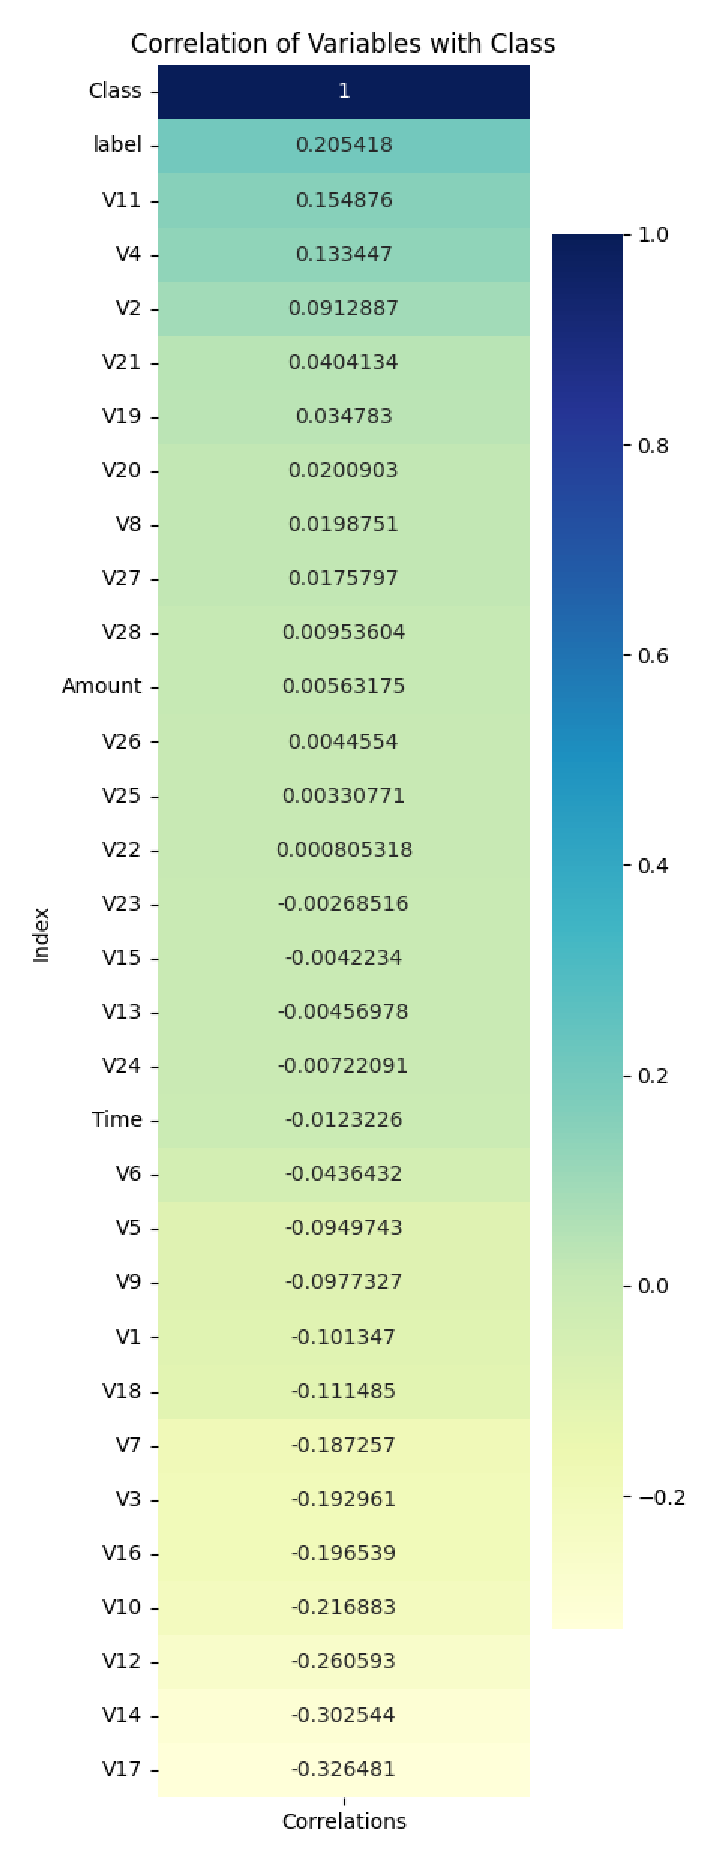
\includegraphics[height=0.5\textheight]{figures/correlation.eps}
	\caption{\DIFaddFL{correlation heat plot}}
	\label{fig:correlation}
\end{figure}
\DIFaddend 




\DIFdelbegin \DIFdel{The authors would like to thank \ldots
}\DIFdelend \DIFaddbegin \section{\DIFadd{Experiment}} \label{sec-experiment}
\DIFadd{In the experimental design, we achieved the optimal performance of the model by continuously adjusting parameters. The evaluation of the training set's accuracy and recall mainly involved removing attributes and continuously changing the parameters of the isolation forest.
}

\begin{table}\centering

	\caption{\DIFaddFL{parameter adjustment}}
	\label{tbl:parameter-adjustment}
	\resizebox{\textwidth}{!}{
		\begin{tabular}{cccccc}
			\toprule
			Parameter & Accuarcy & Recall & Parameter & Accuarcy & Recall\\
			\midrule
			none-parameter-adjust & 0.963 & 0.821  & none-parameter-adjust(feature \_delete) & 0.953 & 0.663 \\
			n\_estimators-adjust(220) & 0.981 & 0.722  & n\_estimators-adjust(feature \_delete)(140) & 0.980 & 0.520 \\
			n\_features-adjust(11) & 0.981 & 0.750  & n\_features-adjust(feature \_delete)(11) & 0.981 & 0.522 \\
			max\_samples-adjust & 0.981 & 0.829  & nmax\_samples-adjust(feature \_delete) & 0.980 & 0.634\\
			\bottomrule
		\end{tabular}
	}
\end{table}

\cref{tbl:parameter-adjustment} \DIFadd{displays the accuracy and recall rates under various parameter adjustments. From the table, it can be observed that the recall rate deteriorates after removing some features. This implies that although these features may exhibit negative correlations with the outcome, they should not be indiscriminately deleted. By iteratively trying different parameter combinations, we ultimately identified the optimal parameters.
}

\cref{fig:fig_n_estimators} \DIFadd{and }\cref{fig:n_features-adjust}  \DIFadd{and }\cref{fig:max_samples-adjust} \DIFadd{are visualizations of specific parameter adjustments. 
}\begin{figure}
	\centering
	\subfigure[n\_estimators-adjust]{
		\begin{minipage}[b]{0.4\textwidth}
			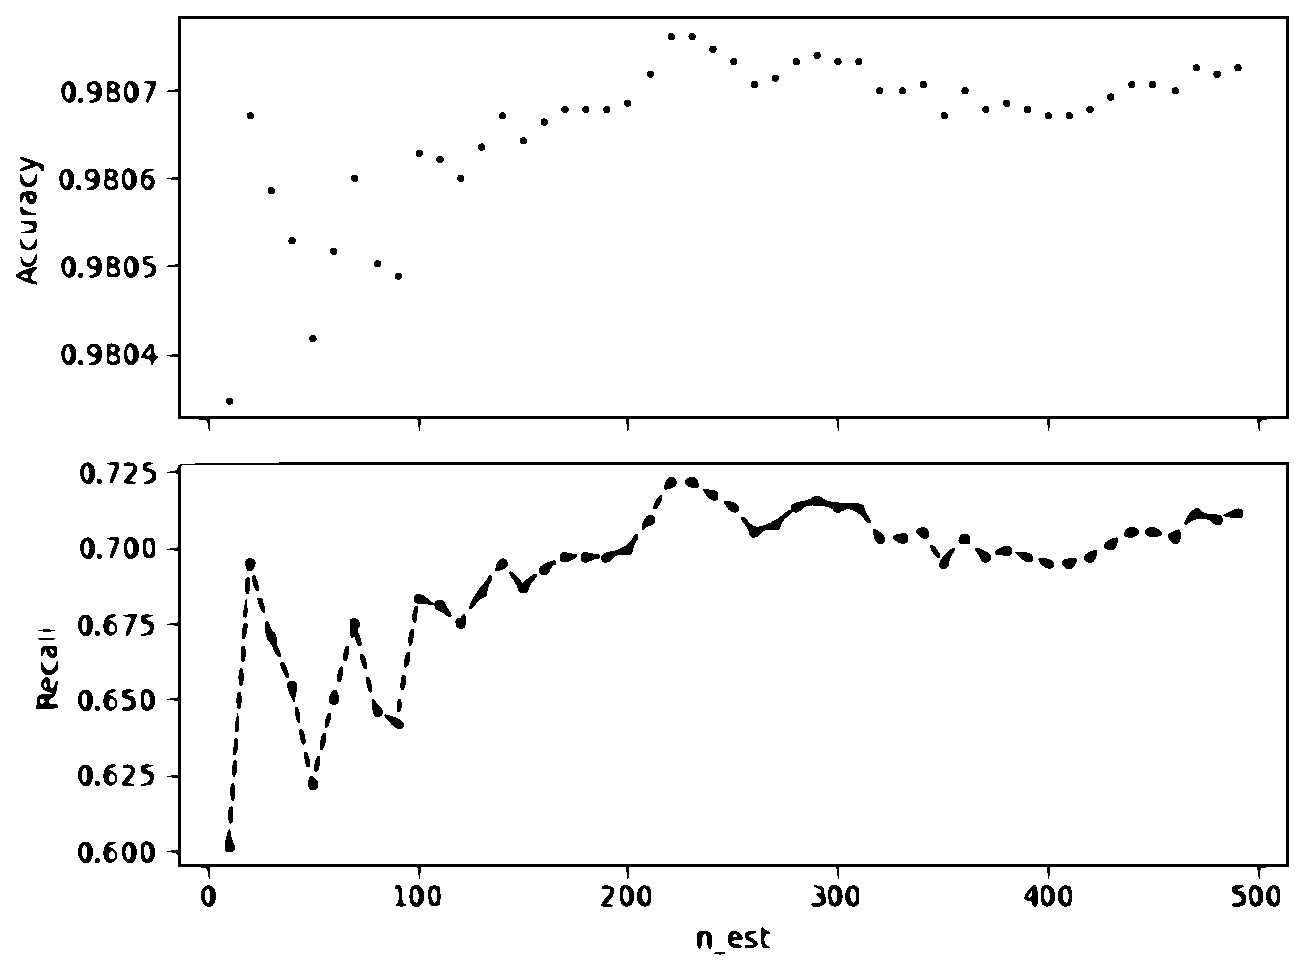
\includegraphics[width=1\textwidth]{figures/n_est_node.eps}
		\end{minipage}
		\label{fig:hor_2figs_1cap_2subcap_1}
	}
	\subfigure[n\_estimators-adjust (feature\_delete)]{
		\begin{minipage}[b]{0.4\textwidth}
			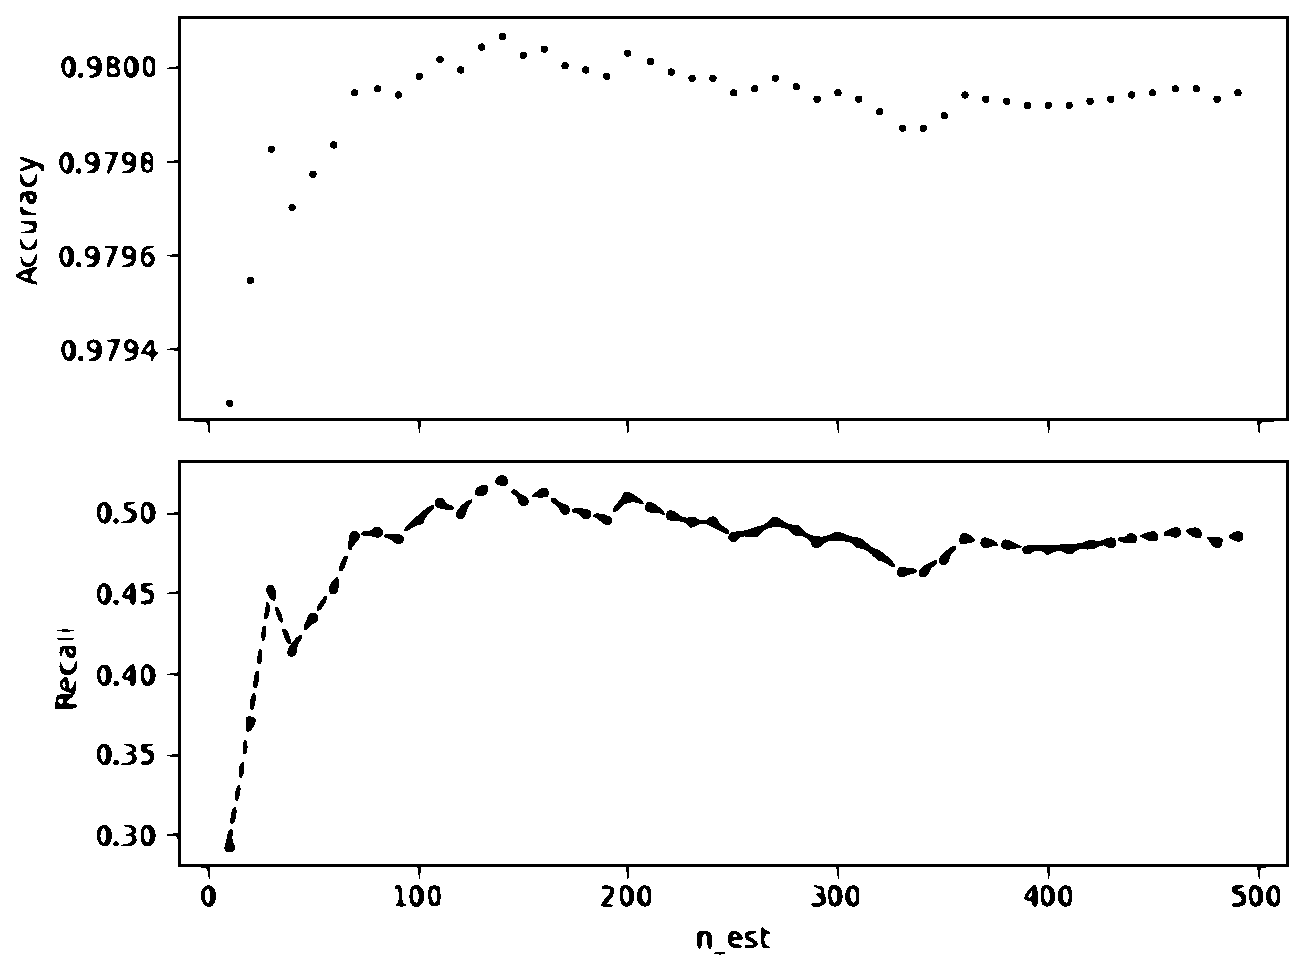
\includegraphics[width=1\textwidth]{figures/n_est.eps}
		\end{minipage}
		\label{fig:hor_2figs_1cap_2subcap_2}
	}
	\caption{\DIFaddFL{n\_estimators-adjust}}
	\label{fig:fig_n_estimators}
\end{figure}

\begin{figure}
	\centering
	\subfigure[n\_features-adjust]{
		\begin{minipage}[b]{0.4\textwidth}
			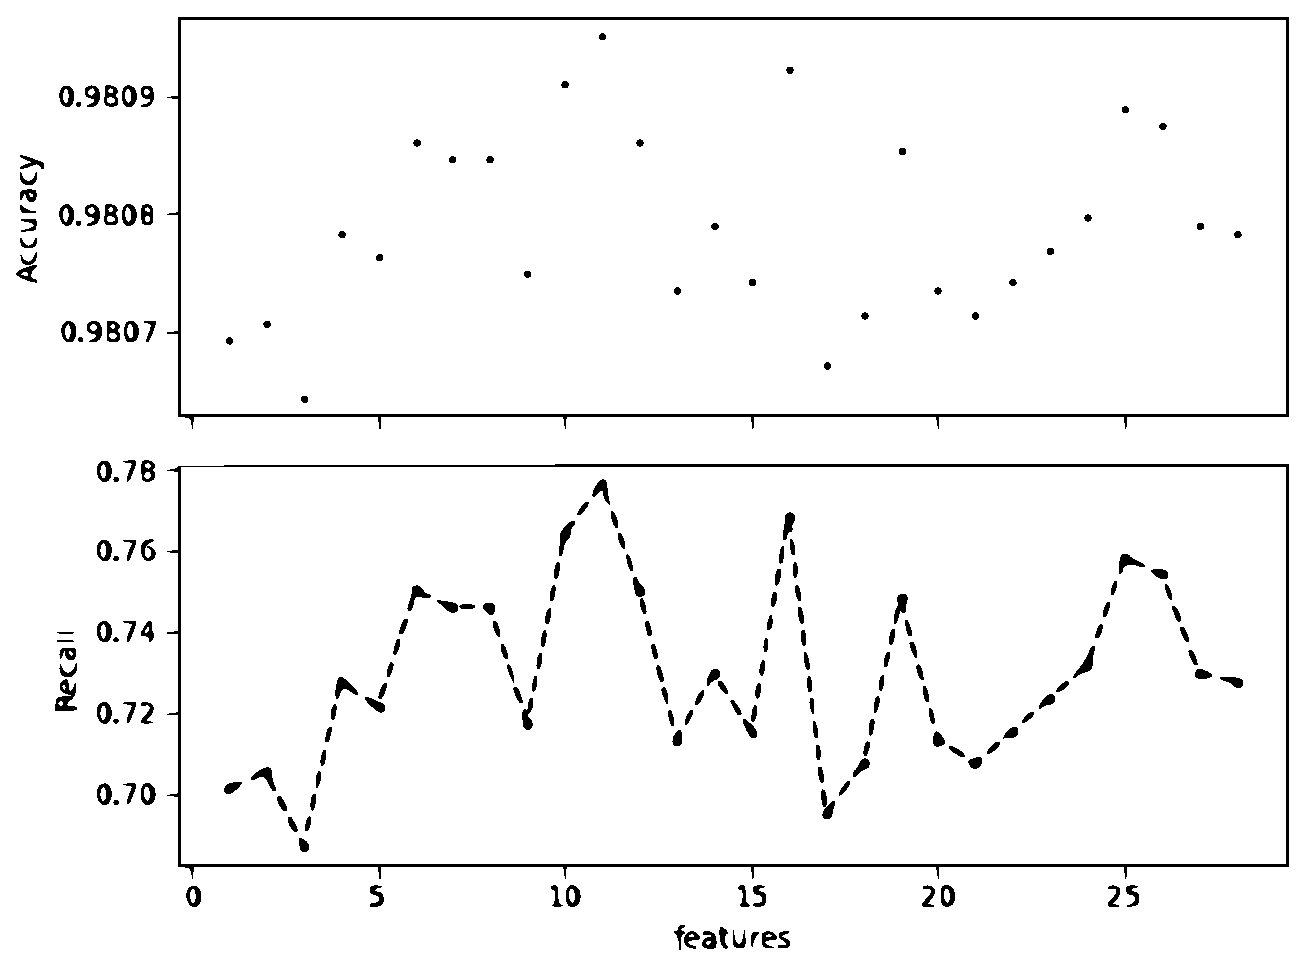
\includegraphics[width=1\textwidth]{figures/feature_nodelete.eps}
		\end{minipage}
		\label{fig:hor_2}
	}
	\subfigure[n\_features-adjust (feature\_delete)]{
		\begin{minipage}[b]{0.4\textwidth}
			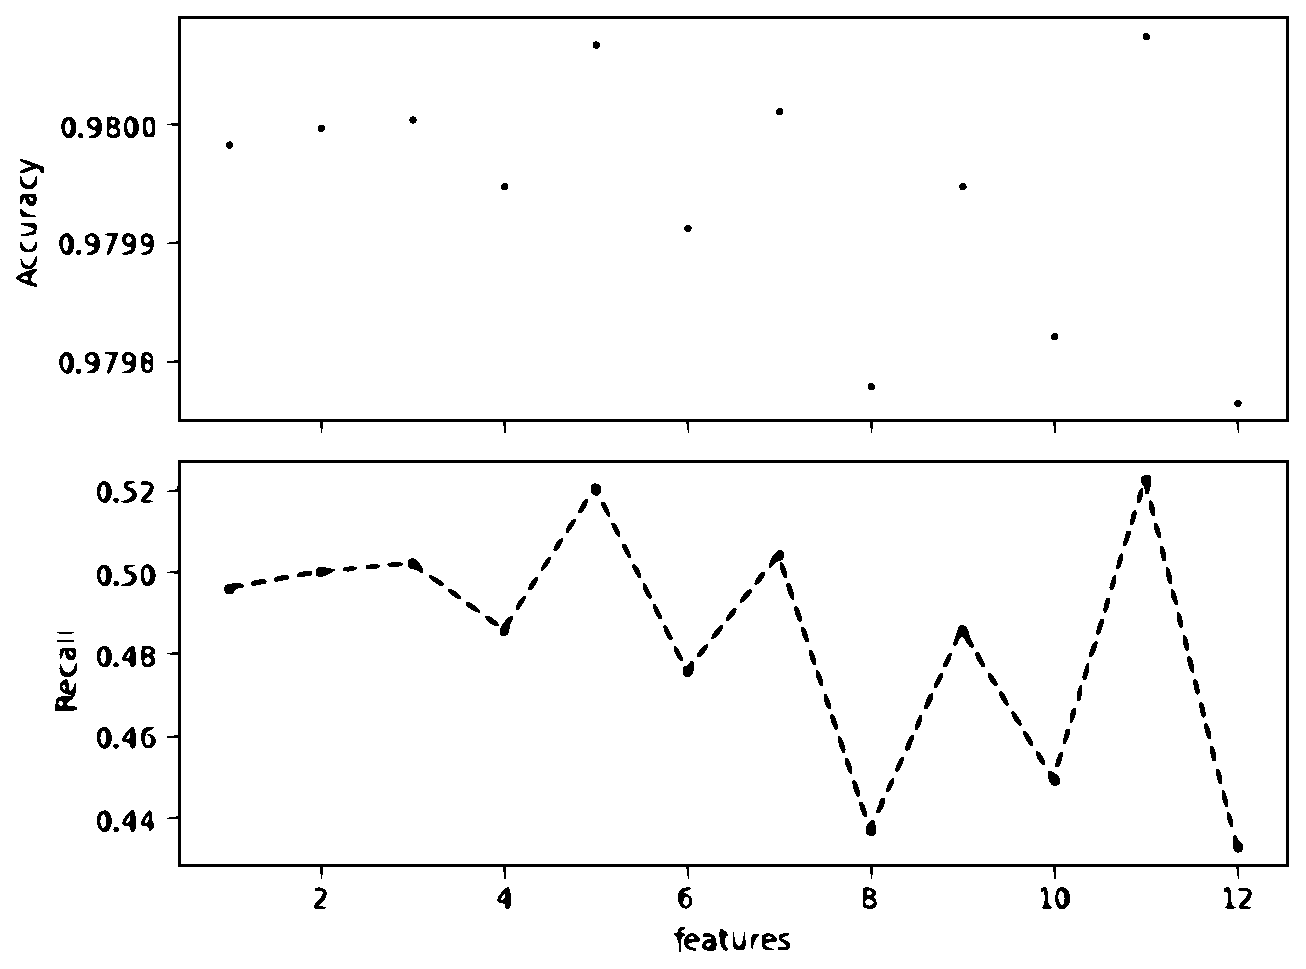
\includegraphics[width=1\textwidth]{figures/feature.eps}
		\end{minipage}
		\label{fig:hor}
	}
	\caption{\DIFaddFL{n\_efeatures-adjust}}
	\label{fig:n_features-adjust}
\end{figure}

\begin{figure}
	\centering
	\subfigure[max\_samples-adjust]{
		\begin{minipage}[b]{0.4\textwidth}
			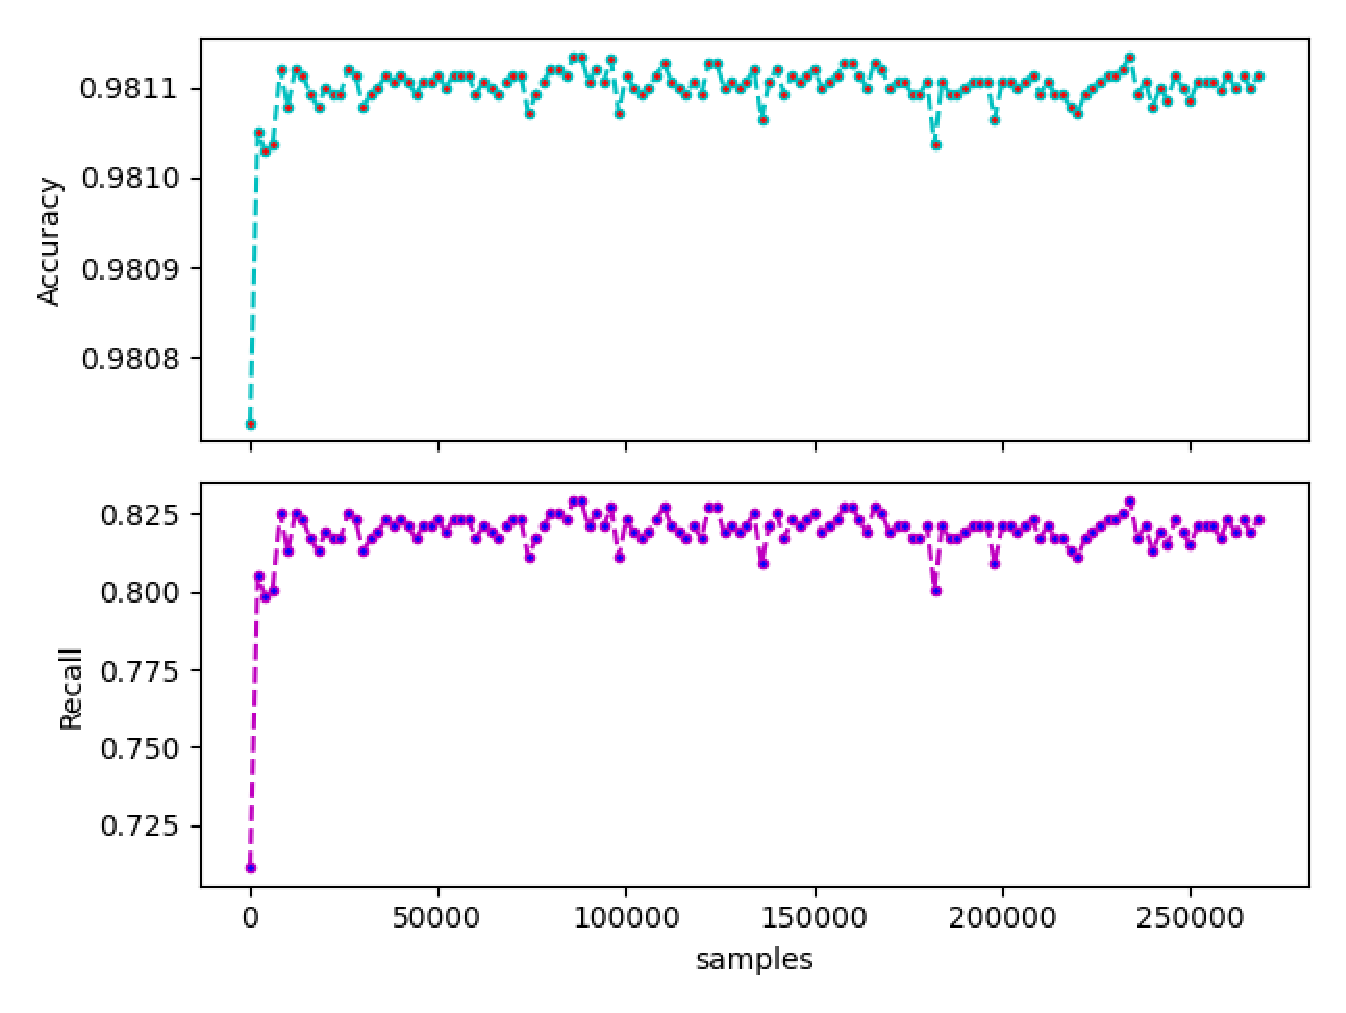
\includegraphics[width=1\textwidth]{figures/max_exampleN.eps}
		\end{minipage}
		\label{fig:h}
	}
	\subfigure[max\_samples-adjust (feature\_delete)]{
		\begin{minipage}[b]{0.4\textwidth}
			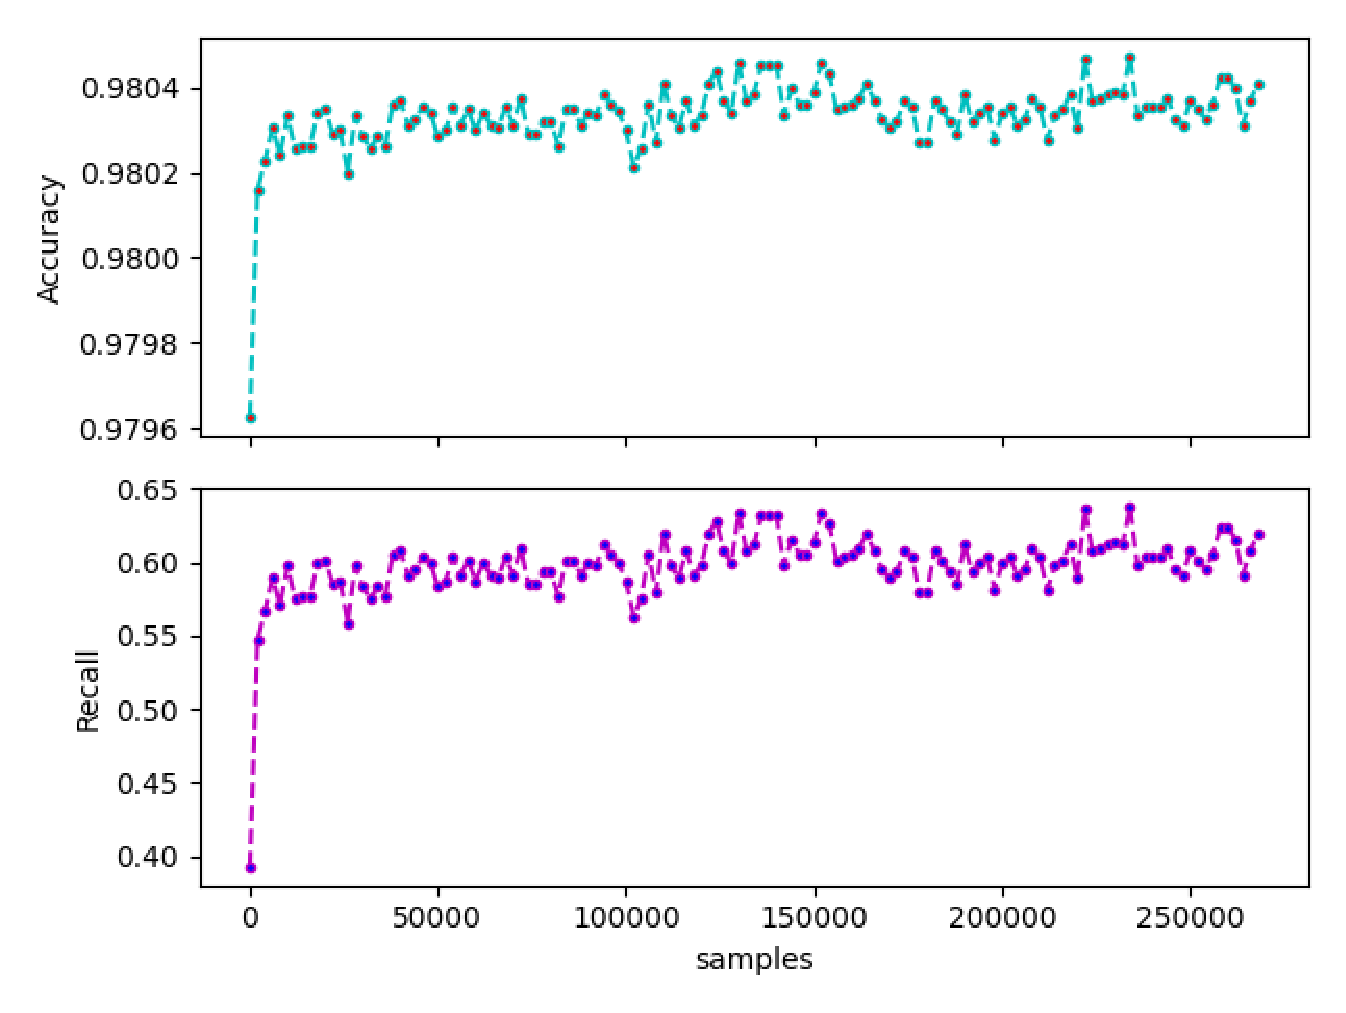
\includegraphics[width=1\textwidth]{figures/max_example.eps}
		\end{minipage}
		\label{fig:ho}
	}
	\caption{\DIFaddFL{max\_samples-adjust}}
	\label{fig:max_samples-adjust}
\end{figure}

\section{\DIFadd{Conclusions}} \label{sec-conclusions}

\DIFadd{The detection of credit card fraud data was achieved through Isolation Forest, and by continuously adjusting the parameters of the algorithm, a high level of accuracy and recall was ultimately reached, at 0.98 and 0.8, respectively.
}

\DIFadd{However, a notable drawback of this method is the lack of a more in-depth analysis of attributes. This could mean that in the data preprocessing stage or feature selection process, there was insufficient exploration, understanding, and utilization of attribute information relevant to fraud. While optimizing the accuracy and recall of the model is undoubtedly important, equal attention should also be given to the importance and correlation of attributes, as well as their role in fraud detection.
}\DIFaddend 




% ----------------------------------------------------------------
\DIFdelbegin %DIFDELCMD < \newpage
%DIFDELCMD < \bibliography{tuliplab,yourbib}
%DIFDELCMD < %%%
%DIF <  TODO: you should change this yourbib into a proper bib file name
%DIFDELCMD < \bibliographystyle{plainnat}
%DIFDELCMD < %%%
\DIFdelend %=================================================================
\DIFdelbegin %DIFDELCMD < 

%DIFDELCMD < \listoftodos
%DIFDELCMD < %%%
\DIFdelend 


\end{document}

